
\documentclass[11pt]{article}

\usepackage[margin=1in]{geometry}
\usepackage{graphicx}
\usepackage{booktabs}
\usepackage{array}
\usepackage{amsmath}
\usepackage{hyperref}
\usepackage{xcolor}
\usepackage{float}
\usepackage{tikz}
\usetikzlibrary{arrows.meta, positioning, shapes.geometric, fit}

\hypersetup{
    colorlinks=true,
    linkcolor=blue,
    urlcolor=blue,
    citecolor=blue
}

\title{\textbf{Face-to-BMI Prediction using Transfer Learning and Multi-Task Deep Learning}}
\author{Anuradha Rakh}
\date{\today}

\begin{document}

\maketitle

\begin{abstract}
This project develops an end-to-end machine learning system for predicting Body Mass Index (BMI) from facial images. The work is inspired by the Face-to-BMI paper, which reported an overall Pearson correlation of 0.65 using VGG-Face features and support vector regression. We implemented and compared four deep learning models: a VGG16 baseline, a ResNet50 multi-task model, an EfficientNet fine-tuning model, and a ResNet50 BMI-only ablation. The best model was the ResNet50 multi-task architecture, which jointly predicted BMI and gender, achieving a Pearson correlation of 0.6811 and surpassing the reported benchmark. The project also includes a Streamlit-based user interface for image upload, webcam input, model selection, and BMI prediction display.
\end{abstract}

\section{Introduction}

Body Mass Index (BMI) is a widely used measure for estimating body weight status using height and weight. Traditional BMI measurement requires explicit height and weight information, but recent advances in computer vision suggest that facial appearance may contain useful visual signals correlated with BMI. Facial adiposity, jaw structure, cheek fullness, and other visual features may provide predictive information.

The goal of this project is to build a practical deep learning system that predicts BMI from face images. The project follows a research-style workflow: dataset preparation, model development, training, evaluation, hyperparameter tuning, ablation study, and deployment through a web interface.

\section{Problem Statement}

Given an input facial image, the objective is to predict a continuous BMI value:

\[
f(x) \rightarrow \hat{y}_{BMI}
\]

where \(x\) is the input image and \(\hat{y}_{BMI}\) is the predicted BMI. This is a regression problem, not a classification problem.

The main evaluation metric is Pearson correlation coefficient \(r\), which measures how strongly the predicted BMI values correlate with the true BMI values.

\section{Dataset}

The dataset contains facial images and metadata including BMI, gender, train-test split indicator, and image filename.

\subsection{Dataset Format}

The CSV file contains the following columns:

\begin{itemize}
    \item \texttt{bmi}: continuous BMI label
    \item \texttt{gender}: Male or Female
    \item \texttt{is\_training}: train/test split indicator
    \item \texttt{name}: image filename
\end{itemize}

\subsection{Dataset Statistics}

\begin{table}[H]
\centering
\begin{tabular}{lr}
\toprule
\textbf{Metric} & \textbf{Value} \\
\midrule
Total CSV rows & 4206 \\
Valid usable images & 3962 \\
Training samples & 3210 \\
Testing samples & 752 \\
Male samples & 2354 \\
Female samples & 1608 \\
\bottomrule
\end{tabular}
\caption{Final dataset statistics after removing missing images.}
\end{table}

\section{Overall Project Pipeline}

Figure~\ref{fig:pipeline} shows the complete project workflow.

\begin{figure}[H]
\centering
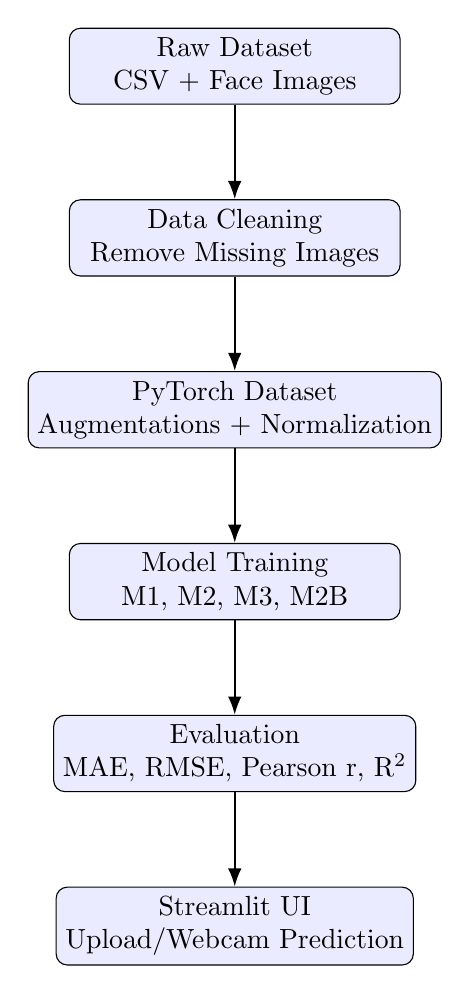
\begin{tikzpicture}[
    node distance=1.2cm,
    box/.style={rectangle, rounded corners, draw=black, fill=blue!8, minimum width=4.2cm, minimum height=0.85cm, align=center},
    arrow/.style={-{Latex}, thick}
]
\node[box] (data) {Raw Dataset\\CSV + Face Images};
\node[box, below=of data] (prep) {Data Cleaning\\Remove Missing Images};
\node[box, below=of prep] (loader) {PyTorch Dataset\\Augmentations + Normalization};
\node[box, below=of loader] (train) {Model Training\\M1, M2, M3, M2B};
\node[box, below=of train] (eval) {Evaluation\\MAE, RMSE, Pearson r, R\textsuperscript{2}};
\node[box, below=of eval] (deploy) {Streamlit UI\\Upload/Webcam Prediction};

\draw[arrow] (data) -- (prep);
\draw[arrow] (prep) -- (loader);
\draw[arrow] (loader) -- (train);
\draw[arrow] (train) -- (eval);
\draw[arrow] (eval) -- (deploy);
\end{tikzpicture}
\caption{End-to-end Face-to-BMI project pipeline.}
\label{fig:pipeline}
\end{figure}

\section{Methodology}

This project uses transfer learning. Instead of training a convolutional neural network from scratch, pretrained models are reused as visual feature extractors. A small task-specific prediction head is added on top of each backbone.

The general model structure is:

\[
\text{Image} \rightarrow \text{Pretrained CNN Backbone} \rightarrow \text{Regression Head} \rightarrow \text{BMI}
\]

\section{Model Architectures}

\subsection{M1: VGG16 Baseline}

The first model uses VGG16 pretrained on ImageNet. The convolutional backbone is frozen, and a dense regression head is trained for BMI prediction.

\begin{figure}[H]
\centering
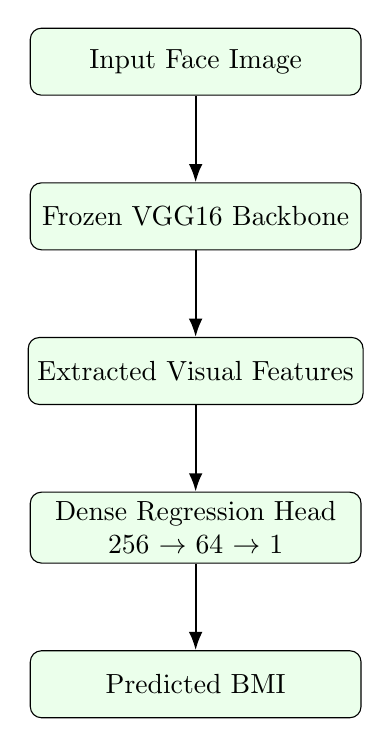
\begin{tikzpicture}[
    node distance=1.1cm,
    box/.style={rectangle, rounded corners, draw=black, fill=green!8, minimum width=4.2cm, minimum height=0.85cm, align=center},
    arrow/.style={-{Latex}, thick}
]
\node[box] (input) {Input Face Image};
\node[box, below=of input] (vgg) {Frozen VGG16 Backbone};
\node[box, below=of vgg] (features) {Extracted Visual Features};
\node[box, below=of features] (head) {Dense Regression Head\\256 $\rightarrow$ 64 $\rightarrow$ 1};
\node[box, below=of head] (output) {Predicted BMI};

\draw[arrow] (input) -- (vgg);
\draw[arrow] (vgg) -- (features);
\draw[arrow] (features) -- (head);
\draw[arrow] (head) -- (output);
\end{tikzpicture}
\caption{M1 VGG16 baseline architecture.}
\end{figure}

\subsection{M2: ResNet50 Multi-Task Model}

The best-performing model uses ResNet50 as a shared backbone. It predicts both BMI and gender. BMI prediction is the primary task, while gender classification is an auxiliary task.

\begin{figure}[H]
\centering
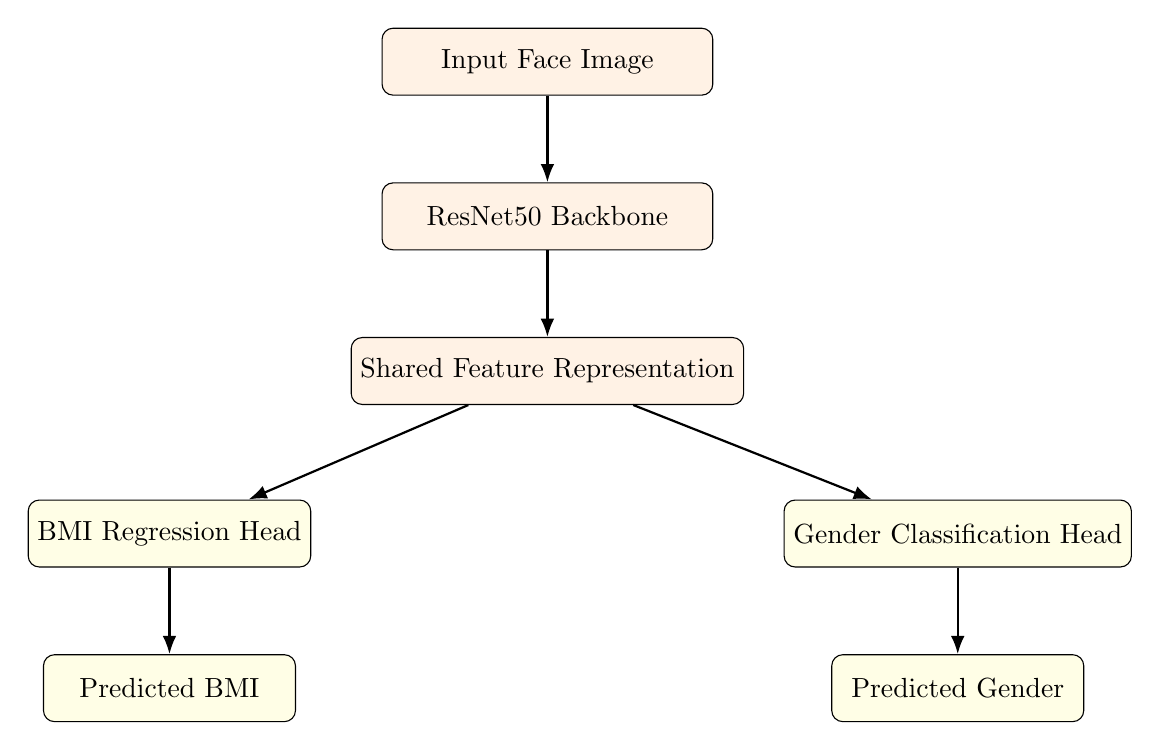
\begin{tikzpicture}[
    node distance=1.1cm,
    box/.style={rectangle, rounded corners, draw=black, fill=orange!10, minimum width=4.2cm, minimum height=0.85cm, align=center},
    smallbox/.style={rectangle, rounded corners, draw=black, fill=yellow!10, minimum width=3.2cm, minimum height=0.85cm, align=center},
    arrow/.style={-{Latex}, thick}
]
\node[box] (input) {Input Face Image};
\node[box, below=of input] (resnet) {ResNet50 Backbone};
\node[box, below=of resnet] (shared) {Shared Feature Representation};
\node[smallbox, below left=1.2cm and 0.5cm of shared] (bmi) {BMI Regression Head};
\node[smallbox, below right=1.2cm and 0.5cm of shared] (gender) {Gender Classification Head};
\node[smallbox, below=of bmi] (bmiout) {Predicted BMI};
\node[smallbox, below=of gender] (genderout) {Predicted Gender};

\draw[arrow] (input) -- (resnet);
\draw[arrow] (resnet) -- (shared);
\draw[arrow] (shared) -- (bmi);
\draw[arrow] (shared) -- (gender);
\draw[arrow] (bmi) -- (bmiout);
\draw[arrow] (gender) -- (genderout);
\end{tikzpicture}
\caption{M2 ResNet50 multi-task architecture.}
\label{fig:m2}
\end{figure}

The total loss is:

\[
L = \lambda_{BMI} L_{BMI} + \lambda_{gender} L_{gender}
\]

where \(L_{BMI}\) is the regression loss and \(L_{gender}\) is the gender classification loss.

The final tuned configuration used:

\begin{itemize}
    \item Epochs: 35
    \item Learning rate: 0.00003
    \item Dropout: 0.25
    \item BMI loss weight: 1.0
    \item Gender loss weight: 0.10
\end{itemize}

\subsection{M3: EfficientNet Fine-Tuning}

EfficientNet-B0 was used as a modern CNN backbone. Most layers were initially frozen, while the last three blocks were unfrozen for fine-tuning.

\begin{figure}[H]
\centering
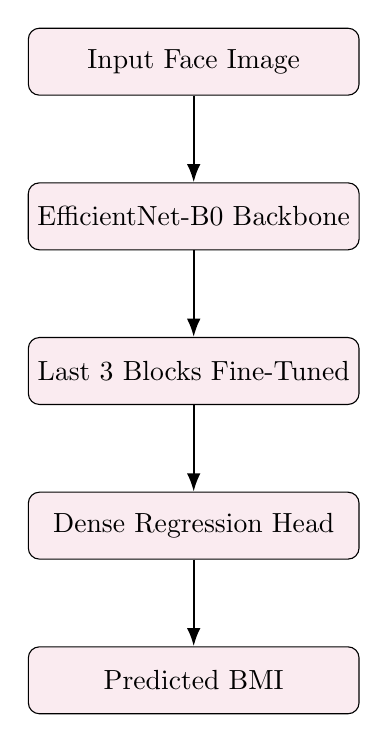
\begin{tikzpicture}[
    node distance=1.1cm,
    box/.style={rectangle, rounded corners, draw=black, fill=purple!8, minimum width=4.2cm, minimum height=0.85cm, align=center},
    arrow/.style={-{Latex}, thick}
]
\node[box] (input) {Input Face Image};
\node[box, below=of input] (eff) {EfficientNet-B0 Backbone};
\node[box, below=of eff] (blocks) {Last 3 Blocks Fine-Tuned};
\node[box, below=of blocks] (head) {Dense Regression Head};
\node[box, below=of head] (output) {Predicted BMI};

\draw[arrow] (input) -- (eff);
\draw[arrow] (eff) -- (blocks);
\draw[arrow] (blocks) -- (head);
\draw[arrow] (head) -- (output);
\end{tikzpicture}
\caption{M3 EfficientNet fine-tuning architecture.}
\end{figure}

\subsection{M2B: ResNet50 BMI-Only Ablation}

The M2B model was created as an ablation study. It uses the same ResNet50 backbone but removes the gender classification branch. This tests whether auxiliary gender supervision improves BMI prediction.

\section{Training Strategy}

The training process used the following steps:

\begin{enumerate}
    \item Load cleaned train/test CSV files.
    \item Apply training image augmentations.
    \item Normalize images using ImageNet statistics.
    \item Train the selected model.
    \item Evaluate on the held-out test set.
    \item Save the checkpoint with the best Pearson correlation.
\end{enumerate}

\begin{figure}[H]
\centering
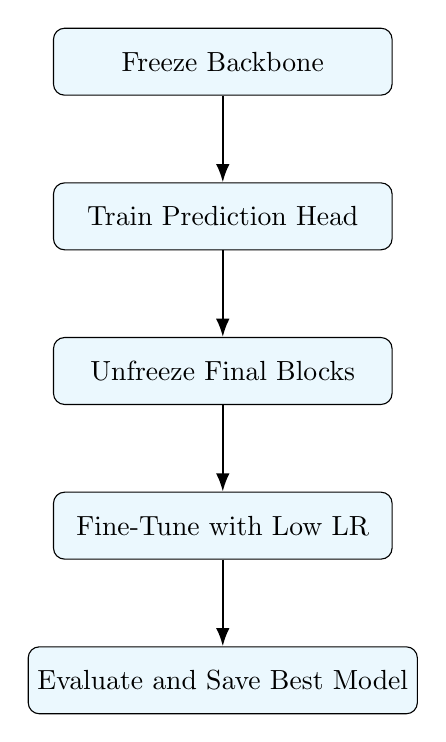
\begin{tikzpicture}[
    node distance=1.1cm,
    box/.style={rectangle, rounded corners, draw=black, fill=cyan!8, minimum width=4.3cm, minimum height=0.85cm, align=center},
    arrow/.style={-{Latex}, thick}
]
\node[box] (freeze) {Freeze Backbone};
\node[box, below=of freeze] (head) {Train Prediction Head};
\node[box, below=of head] (unfreeze) {Unfreeze Final Blocks};
\node[box, below=of unfreeze] (fine) {Fine-Tune with Low LR};
\node[box, below=of fine] (eval) {Evaluate and Save Best Model};

\draw[arrow] (freeze) -- (head);
\draw[arrow] (head) -- (unfreeze);
\draw[arrow] (unfreeze) -- (fine);
\draw[arrow] (fine) -- (eval);
\end{tikzpicture}
\caption{Training and fine-tuning workflow.}
\end{figure}

\section{Evaluation Metrics}

The primary metric is Pearson correlation coefficient:

\[
r = \frac{\sum_i (y_i - \bar{y})(\hat{y}_i - \bar{\hat{y}})}
{\sqrt{\sum_i (y_i - \bar{y})^2}\sqrt{\sum_i(\hat{y}_i - \bar{\hat{y}})^2}}
\]

Additional metrics include:

\begin{itemize}
    \item Mean Absolute Error (MAE)
    \item Root Mean Squared Error (RMSE)
    \item \(R^2\) score
\end{itemize}

\section{Experimental Results}

\begin{table}[H]
\centering
\begin{tabular}{llc}
\toprule
\textbf{Model} & \textbf{Description} & \textbf{Pearson r} \\
\midrule
M1 & VGG16 Baseline & 0.4227 \\
M3 & EfficientNet Fine-Tune & 0.5532 \\
M2B & ResNet50 BMI-Only & 0.5771 \\
M2 & ResNet50 Multi-Task & \textbf{0.6811} \\
\bottomrule
\end{tabular}
\caption{Final model comparison.}
\end{table}

The ResNet50 multi-task model achieved the best result with a Pearson correlation of 0.6811. This surpassed the paper benchmark of 0.65.

\section{Discussion}

The results show that ResNet50 features are more effective than VGG16 features for this task. The multi-task approach slightly outperformed the BMI-only ResNet50 ablation, suggesting that gender supervision acted as a useful regularizer.

EfficientNet improved after tuning but did not outperform ResNet50. This may be due to the limited size of the dataset, sensitivity of EfficientNet to hyperparameters, or the need for stronger face-specific preprocessing.

\section{Streamlit Deployment}

A Streamlit user interface was created for demonstration. The interface supports image upload, webcam input, model selection toggles, gender selection, prediction results, loading spinner, and reset buttons.

\begin{figure}[H]
\centering
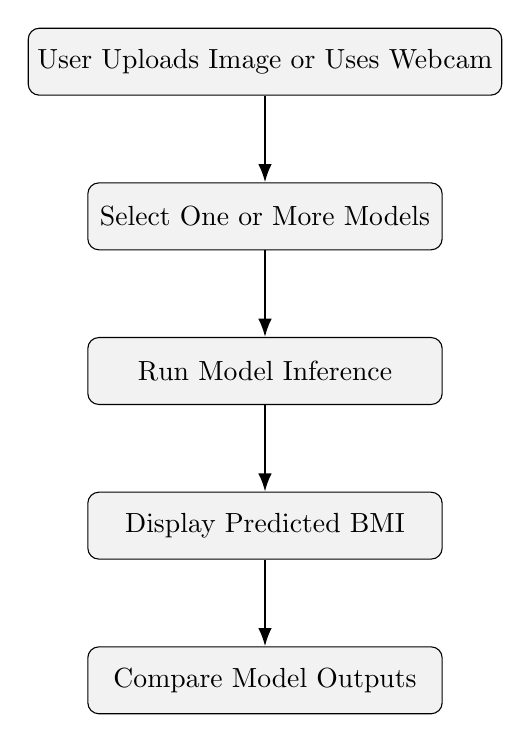
\begin{tikzpicture}[
    node distance=1.1cm,
    box/.style={rectangle, rounded corners, draw=black, fill=gray!10, minimum width=4.5cm, minimum height=0.85cm, align=center},
    arrow/.style={-{Latex}, thick}
]
\node[box] (user) {User Uploads Image or Uses Webcam};
\node[box, below=of user] (select) {Select One or More Models};
\node[box, below=of select] (infer) {Run Model Inference};
\node[box, below=of infer] (display) {Display Predicted BMI};
\node[box, below=of display] (compare) {Compare Model Outputs};

\draw[arrow] (user) -- (select);
\draw[arrow] (select) -- (infer);
\draw[arrow] (infer) -- (display);
\draw[arrow] (display) -- (compare);
\end{tikzpicture}
\caption{Streamlit deployment workflow.}
\end{figure}

\section{Limitations}

Although the final model surpassed the reported benchmark, several limitations remain:

\begin{itemize}
    \item BMI from face alone is noisy and imperfect.
    \item Lighting, pose, age, expression, and image quality affect predictions.
    \item Dataset size is relatively small for deep learning.
    \item BMI is a population-level measure and should not be treated as a complete individual health assessment.
    \item Ethical concerns exist when inferring body-related attributes from images.
\end{itemize}

\section{Future Work}

Future improvements could include:

\begin{itemize}
    \item Face alignment before model input
    \item ArcFace or FaceNet embeddings
    \item Ensemble averaging
    \item Better hyperparameter search
    \item Grad-CAM visualization
    \item Model calibration
    \item More diverse training data
\end{itemize}

\section{Conclusion}

This project built a complete Face-to-BMI prediction system using deep learning. Four models were implemented and compared. The best model, ResNet50 multi-task learning, achieved a Pearson correlation of 0.6811, outperforming the benchmark value of 0.65. The project demonstrates transfer learning, fine-tuning, multi-task learning, model comparison, and deployment through a Streamlit interface.

\section*{References}

Kocabey, E., Camurcu, M., Ofli, F., Aytar, Y., Marin, J., Torralba, A., and Weber, I. Face-to-BMI: Using Computer Vision to Infer Body Mass Index on Social Media. ICWSM, 2017.

\end{document}
